\documentclass[11pt, a4paper, draft]{article}
\usepackage{tmh}
\usepackage{bbm}
\renewcommand{\labelenumi}{\roman{enumi})}
\renewcommand{\phi}{\varphi}

\renewcommand{\P}{\mathbb{P}}
\newcommand{\E}{\mathbb{E}}
\renewcommand{\R}{\mathbb{R}}
\newcommand{\T}{\mathbb{T}}
\newcommand{\Z}{\mathbb{Z}}
\newcommand{\F}{\mathcal{F}}
\newcommand{\Dt}{\Delta t}
\newcommand{\Dv}{\Delta v}
\newcommand{\Dx}{\Delta x}
\newcommand{\dx}{\dif x}
\newcommand{\dt}{\dif t}
\renewcommand{\familydefault}{\sfdefault}
\usepackage[scaled]{helvet}
\setlength{\parindent}{0em}
\setlength{\parskip}{1em}

\usepackage{showkeys}

\title{{\huge Interacting Particle Systems} \\\vspace{1cm} Subtitle}
\author{Thomas M. Hodgson\\ \vspace{0.5cm} Maxwell Institute}
\date{\today}

\begin{document}

	\maketitle
	\newpage
	\tableofcontents
	\listoffigures
	\newpage
	\section{Introduction}
	+++Motivation, particle systems and flocking in biology+++
	\section{The Model}\label{sec:model}
		We here elucidate the model of Butt\`a, Flandoli, Ottobre and Zegarlinski \cite{Butta2019}. This is a Vicsek-type continuum model for an interacting particle system. There are three key parts to this model that together create interaction and ordered motion: a herding function, denoted $G$; an averaging function, denoted $M$; and an interaction function, $\phi$. Each will be described before the full model is introduced. Throughout, we will be considering the phase space distribution function $f_t(x,v)$, where $(x,v) \in \T \times \R$ and $t \in \R$ with $\T \cong \R \backslash \Z \cong S^1$ denoting the unit one-dimensional torus. The distribution function represents the density of particles at time $t$ at a given point in phase space $(x,v)$.
		
		The interaction function, $\phi: \T \to \R $ acts on the smallest scale, between individual points. It is smooth and satisfies the following:
		\begin{align*}
			\phi(x) \geq \epsilon >0, && \phi(x) = \phi(-x), &&& \int_{\T} \phi(x) \dif x = 1.
		\end{align*}
		These are quite natural ways to describe an interaction. The first means that all points interact with each other to some degree. +++ Positivity requires that all interactions are attractive, in contrast to many real-world phenomena, give examples of only attractive systems +++. The second requires symmetry when interacting, and finally the function must have unit integral -- this is only for simplicity and could in fact be any value, so long as it is finite. For example, we may take $\phi \equiv 1$. This will satisfy the above requirements and corresponds to all points interacting an equal amount, regardless of position on the torus. This will create space-homogeneity, which we will return to later.
		
		The function $M:\R \to \R$ takes a weighted average of the interactions across the space.	
		\[ 
			M(t,x) = \frac{\int_{\T}\int_{\R}f_t(y,w)\phi(x-y)w\dif w \dif y}{\int_{\T}\int_{\R}f_t(y,w)\phi(x-y)\dif w \dif y}
		\]
		The interaction function provides the weighting. Note the argument of  $\phi$ is the distance between two points in space and also that $M$ depends on $f_t$. +++The denominator is required in the corresponding particle model to prevent the size of the group of particles from having an effect on the dynamics. It can be thought of as a normaliser. -- Poor explanation.+++
		
		Finally, the herding function $G:\R \to \R$ is chosen such that
		\begin{align*}
			&G(u)=-G(-u),&& {\begin{cases}
								G(u)>u & \text{ if } 0< u <1\\
								G(u)<u & \text{ if } u > 1
				   		   \end{cases}}.
		\end{align*}
		We shall consider three forms of $G$.
		\begin{enumerate}
			\item Step:
			\[
				G(u) = \frac{1+\beta \mathrm{sgn}(u)}{1+\beta}, \qquad \beta > 0	
			\]
			This is the usual choice in the biological literature, with \(\beta = \frac{1}{2}\). It is differentiable everywhere with $G'(u) = \frac{1}{1+\beta}$, except at $u=0$. This discontinuity makes analysis more difficult.
			\item Smooth:
			\[
				G(u) = \frac{\arctan(u)}{\arctan(1)}
			\]
			Here we get a much smoother curve that is everywhere differentiable. However the gradient isn't very steep and there is no way to control the shape of the curve.
			\item Sigmoid:
			\[
				G(u) = \frac{2}{1+\mathrm{e}^{-\alpha u}} - 1 , \qquad \alpha >0
			\]
			The sigmoid herding function provides a middle ground between the previous two. It is smooth, but can be made as sharp as required by adjusting the parameter $\alpha$. However note that it only satisfies second requirement above in the limit as $\alpha \to \infty$ as the function is bounded above by 1.
		\end{enumerate}
		During the analysis, we will use the smooth herding function for its amenability. The role of $G$ is to herd the mean velocity towards a fixed value -- in this case plus or minus one. How it does so will become clearer when we discuss the dynamics of the model.
		
		We now have all the necessary ingredients to give the full continuum model. The evolution of the distribution is described by
		\begin{equation}\label{eq:fullPDE}
			\partial_t f_t(x,v) = -v\partial_x f_t(x,v)  +\partial_v v f_t(x,v) - \partial_v \left[ G(M(t,x))f_t(x,v)\right] + \sigma \partial_{vv}f_t(x,v),
		\end{equation}
		where $\sigma > 0$ is a constant describing the rate of diffusion. At its heart, this is just an advection-diffusion equation. The first term illustrates the movement around the torus, the second describes a damping effect and the fourth gives a diffusive effect in velocity. The third term is where the interest lies as it contains all the information on interaction and herding.
		
		\section{Dynamics}\label{sec:dynamics}
		To better understand the dynamics of \eqref{eq:fullPDE}, first let $G\equiv0$. This removes any interaction between particles and the equation becomes
		\begin{equation}\label{eq:OU_FPE}
			\partial_t f_t(x,v) = -v\partial_x f_t(x,v) +\partial_v vf_t(x,v) + \sigma \partial_{vv}f_t(x,v).
		\end{equation}
		This is the Fokker-Planck equation for the following system:
		\begin{equation}\label{eq:2d_OU}\begin{cases}
			\dif x_t = v_t\dif t\\
			\dif v_t = -v_t\dif t + \sqrt{2\sigma} \dif W_t. 
		\end{cases}	\end{equation}
		Here, $W_t$ is a standard one-dimensional Wiener process. We recognise this as overdamped Langevin dynamics, and so we can exactly calculate the unique invariant measure. To do so it is necessary to solve $\partial_t \rho_t = 0$, that is, when is the density not changing in time. The evolution in $v$ is described by an Ornstein-Uhlenbeck process so it is known that the unique stationary distribution is Gaussian with mean $1$ and variance $\sigma$. The position $x$ depends only on $v$ with no noise. There is no reason to assume any sort of mean reverting behaviour and expect the density to spread out uniformly on the torus. A guess at the solution would then be $\rho (x,v) = \frac{1}{2\pi}\exp(\frac{-v^2}{2})$, with some normalising constant. Notice that this equation does not depend on $x$. By substitution into the stationary Fokker-Planck equation, this is indeed a solution.
        
        Similarly, when $G\not\equiv 0$ the density $f_t(x,v)$ of \eqref{eq:fullPDE} is the Fokker-Planck equation of the two dimensional SDE,
		    \begin{equation}\label{eq:McK_V}\begin{cases}
		    \dif x_t = v_t\dif t\\
		    \dif v_t = \left[G(M(t,x_t))-v_t\right] \dif t + \sqrt{2\sigma} \dif W_t. 
			\end{cases} \qquad  (x_t,v_t) \in \T \times \R
			\end{equation}
		This is a McKean-Vlasov equation as the function $M(t,x_t)$ conceals a dependence on the law of the process. 
        \[
            M(t,x) = \frac{\E\left[ v'_t \phi(x-x'_t)\right]}{\E\left[\phi(x-x'_t)\right]}
        \]
        The pair $(x'_t,v'_t)$ is a random variable equal in distribution to $(x_t,v_t)$. This representation of $M(t,x)$ is the same as the one given previously, however in this setting it is natural to use expectation notation over integrals. To illustrate the necessity of introducing another random variable, albeit one that is equal in law, consider the case when the interaction function is the indicator on the interval $[-b,b]$, $\phi(x) = \mathbbm{1}_{[-b,b]}(x)$. This does not meet the requirements in Section \ref{sec:model}, in particular it is neither strictly positive nor does it have unit integral. 
        \begin{align*}
            M(t,x) &=  \frac{\int_{\T}\int_{\R}f_t(y,w)\phi(x-y)w\dif w \dif y}{\int_{\T}\int_{\R}f_t(y,w)\phi(x-y)\dif w \dif y}\\
            &=  \frac{\int_{\T}\int_{\R}f_t(y,w) \mathbbm{1}_{[-b,b]}w\dif w \dif y}{\int_{\T}\int_{\R}f_t(y,w) \mathbbm{1}_{[-b,b]}\dif w \dif y}\\
            &= \frac{\E\left[ v'_t \mathbbm{1}_{[-b,b]}\right]}{\P(x' \in \left[x-b,x+b\right])}\\
            &= \E\left[ v'_t|x' \in [x-b,x+b] \right]
        \end{align*}
        It makes no sense to consider $\P(x \in [x-b,x+b])$ as it is always equal to one so the auxiliary variable $(x'_t,v'_t)$ is used. +++More detail?+++ This calculation also illustrates how $\phi$ describes the interaction or `where to look' while $M$ acts as a average velocity of the points `within range'. The transport term, $\partial_v\left( \left[ v-G(M(t,x))\right]f_t(x,v)\right)$ then acts to change the velocity towards the local average given by $M$. It is in this sense that $G$ is the herding function `herding' the system towards a common velocity.
        
        The McKean-Vlasov representation of the system is also the weak limit of an $N$-body particle system described by
        \begin{equation}\label{eq:full_particle}\begin{cases}
            \dif x^{i,N}_t = v^{i,N}_t\dif t\\
            \dif v^{i,N}_t = -v^{i,N}_t\dif t + G\left(\frac{\frac{1}{N}\sum_{j=1}^N \phi(x_t^{i,N} - x_t^{j,N})v^{j,N}_t  }{\frac{1}{N}\sum_{j=1}^N \phi(x_t^{i,N} - x_t^{j,N})}\right)\dif t + \sqrt{2\sigma} \dif W^i_t 
            \end{cases}, \qquad  i = 1,\dots,N.
        \end{equation}
        This gives another view of the full system \eqref{eq:fullPDE}, and one that is particularly amenable to analysis. It also allows a more intuitive view of the system -- rather than thinking of how a density changes over time, we can think of particles moving around a torus and interacting according to $\phi$.
        
        \subsection{Invariant Measures under Space Homogeneity}
        Thus far, we have found the invariant measure for only the rather uninteresting case when $G \equiv 0$. To progress further, we must simplify the system. One way to do this is to impose that the density does not depend on the position in space and set $\phi \equiv 1$. The weighted local average velocity $M$ becomes neither local nor weighted. In the particle system, this means that each particle interacts with every other particle, irrespective of the distance between them. Indeed,
        \begin{align*}
            M(t,x) =&  \frac{\int_{\T}\int_{\R}f_t(y,w)\phi(x-y)w\dif w \dif y}{\int_{\T}\int_{\R}f_t(y,w)\phi(x-y)\dif w \dif y}\\
            =&  \frac{\int_{\T}\int_{\R}f_t(y,w)w\dif w \dif y}{\int_{\T}\int_{\R}f_t(y,w)\dif w \dif y}\\
            =& \int_{\T}\int_{\R}f_t(y,w)w\dif w \dif y\\
            :=& \langle w \rangle_{f_t}.
        \end{align*}
        So the weighted local average velocity is just the average of the distribution $f_t(v)$ or equivalently, the average velocity of all particles in the system. The evolution is then described by
        \begin{equation}\label{eq:space_hom_PDE}
            \partial_t f_t(v) = \partial_v vf_t(v) - \partial_v G(\langle w \rangle_{f_t})f_t(v) + \sigma \partial_{vv} f_t(v).
        \end{equation}
        The above problem's well-posedness can be shown as follows. Let
        \[
            h_t(v) = f_t(u),\text{ where } u = v + \int_0^t G(\langle w\rangle_{f_t}) \dif s.
        \]
        To find an equation that $h_t(v)$ solves, we use the chain rule.
        \begin{align*}
            \partial_t f_t(u) &= \partial_t f_t(u) +  G(\langle w\rangle_{f_t})\partial_v f_t(u) && \text{as   } \pd{g}{v} = 1, \pd{g}{t} = G((\langle w\rangle_{f_t})\\
            &=\partial_v vf_t(u) - \partial_v G(\langle w \rangle_{f_t})f_t(u) + \sigma \partial_{vv} f_t(u) + G(\langle w\rangle_{f_t})\partial_v f_t(u) &&\text{as  } f_t \text{ solves } \eqref{eq:space_hom_PDE}\\
            &=\partial_v vh_t(v) + \sigma \partial_{vv} h_t(v) , \qquad h_0(v) =f_0(v).
        \end{align*}
        So $h_t$ solves the Fokker-Planck equation for the one-dimensional Ornstein-Uhlenbeck process which is well posed +++cite+++. Therefore the solution $f_t(v)$ of \eqref{eq:space_hom_PDE} exists and is unique given initial data. To find invariant measures of this evolution, set the transient term to zero and solve the remaining PDE, which can be written in gradient form. First note that if $G\equiv 0$, this system for $f_t$ is the same as that for $h_t$, and so has a unique invariant measure $\mathcal{N}(0,\sigma)$. When the herding function is non-zero, other measures are also stationary as we will now show. For brevity, we omit the dependence on $v$ of $f$ and write $\langle w \rangle_{f_t} = M_1$. The latter is natural as it denotes the first moment of the distribution.
        \begin{align*}
            &\partial_v\left[(-G(M_1) +v) f + \sigma \partial_v f \right] = 0\\
            \implies& (-G(M_1) +v) f + \sigma \partial_v f = C_1
        \end{align*}
        This ODE is solvable and gives 
        \[
            f(v) = C_2\exp\left(\frac{2G(M_1)v - v^2}{2\sigma} \right). 
        \]
        Applying the constraint $\int_\R f(w)\dif w = 1$ gives $C_2 = \exp(-G^2(M_1))/\sqrt{2\pi\sigma}$. +++note here this is a Gaussian with mean $G(M_1)$? Immediately implies that $M_1 = G(M_1)$ without need for integration +++ Furthermore, from the definition of space average,
        \begin{align*}
            M_1 :=& \int_\R wf(w) \dif w\\ 
            =& \int_\R \frac{w\exp(-G^2(M_1))}{\sqrt{2\pi\sigma}} \exp\left(\frac{2G(M_1)v - v^2}{2\sigma} \right)\\ 
            =& \int_\R \frac{w}{\sqrt{2\pi\sigma}} \exp\left(\frac{ - (v-G(M_1))^2}{2\sigma} \right)\\
            =& G(M_1)
        \end{align*}
        Using the smoothed version of the herding function from Section \ref{sec:model} gives $G(M_1) = 0, \pm 1$. Substituting this into our expression for $f$ gives three invariant measures:
        \begin{align*}
            \rho_0 &= \frac{1}{\sqrt{2\pi\sigma}}\exp\left(-\frac{v^2}{2\sigma} \right), && \rho_{\pm} = \frac{1}{\sqrt{2\pi\sigma}}\exp\left(-\frac{(v\pm 1)^2}{2\sigma}\right).
        \end{align*}
        These are Gaussian densities with mean $0, \pm 1$ and variance $\sigma$.
        
        We have found three invariant measures for the evolution \eqref{eq:space_hom_PDE}, however whether the system will converge to these distributions given initial data remains to be settled. In the space homogeneous case it is possible to close equations on the moments of the distribution. Let $M_n = \int_\R v^n f_t(v) \dif v$ denote the n$^\text{th}$ moment of the distribution $f_t(v)$. Then
        \begin{align*}
            \partial_t M_n(t) &= \int_{\R}v^n \partial_t  f_t(v) \dif v\\
            &= - \int_{\R}v^n \partial_v G(M_1)f_t(v) \dif v + \int_{\R}v^n \partial_v vf_t(v) \dif v + \sigma \int_{\R}v^n \partial_vv f_t(v) \dif v,
        \end{align*}
        as $f_t$ solves the space-homogeneous PDE \eqref{eq:space_hom_PDE}. Using integration by parts and simplifying gives, for the first three moments,
        \begin{align*}
            \dot{M}_0 &= 0,\\
            \dot{M}_1 &= G(M_1) - M_1,\\
            \dot{M}_2 &= 2\lbrack M_1G(M_1) - M_2 + \sigma\rbrack.
        \end{align*}
        The first tells us there is no change in the zeroth moment over time, that is probability is conserved. The equation for the first moment has equilibria at -1, 0 and 1 for the smoothed choice of $G$. Figure +++ref+++ shows the phase plane diagram for this ODE. It shows that given any initial data with positive average velocity, the first moment will converge to one. By symmetry, the same is true for negative initial data, the mean will converge towards negative one. It also shows that mean zero is an unstable equilibrium -- a slight perturbation will move the system from random movement to ordered motion.
        \begin{figure}
            \centering
            %\includegraphics[width=0.7\linewidth]{}
            \caption{Phase plane of the first  +++(and second?)+++ moment ODE}
            \label{fig:M1_phase}
        \end{figure}
        To find the convergence of the variance, we must look at the difference between the second moment and the square of the first.
        \begin{align*}
            \od{}{t}\lbrack M_2 - M_1^2\rbrack &= \dot{M}_2 - 2M_1\dot{M}_1\\
            &= 2\lbrack G(M_1)M_1 - M_2 +\sigma\rbrack - 2M_1\lbrack G(M_1) - M_1\rbrack\\
            &= -2M_2 +2\sigma + 2M_1^2\\
            &= 2\lbrack M_2 - M_1^2 -\sigma\rbrack             
        \end{align*}
        Solving this ODE gives $M_2-M_1^2 = \sigma +(\sigma_0-\sigma)\mathrm{e}^{-2t}$, where $\sigma_0$ is the variance of the initial data $f_0$. Then as $t \to \infty$, it can be seen that the system forgets its initial data and tends towards a distribution with variance $\sigma$.
        
        The equations on the moments have shown that the system indeed converges to a measure with mean $\pm 1$ and variance $\sigma$ however this is not sufficient to conclude that they are Gaussian. To do so requires closing equations on all the cumulants of the distribution. It can be shown that these vanish for all cumulants of order greater than three and so the system indeed converges towards the invariant measures found by solving the space-homogeneous PDE \eqref{eq:space_hom_PDE}. This means that irrespective of initial data, we expect all particles to move on average in the same direction with the same velocity -- a phenomenon known as unconditional flocking. The only exception is when the initial data has mean zero. In this case the system will converge to the Gaussian with mean zero, corresponding to disordered motion. +++not a great explanation+++
        
        The dynamics of the space-homogeneous system have thus been fully characterised analytically. We will now turn our attention to the particle model in this case.
    \subsubsection{Particle System Dynamics}
        As the particle system approximates the McKean-Vlasov SDE, whose density solves the PDE \eqref{eq:space_hom_PDE}, one would expect that it behaves in entirely the same way. This is in fact not the case, as we will now show. Consider the particle system \eqref{eq:full_particle} in the space-homogeneous case,
        \begin{equation}\label{eq:hom_particle}
            \dif v^{i,N}_t = G\left(\frac{1}{N}\sum_{j=1}^n v^{j,N}_t\right)\dif t-v^{i,N}_t \dif t + \sqrt{2\sigma} \dif W^i_t
        \end{equation}
        It has been shown for the kinetic model that the invariant measures have mean zero and $\pm 1$ when we consider a smoothed herding function. Here we will show that the space-homogeneous particle model only admits invariant measures with mean zero for any herding function satisfying the earlier requirements in Section \ref{sec:model}, before finding analytic forms for the functions we will be using. First note that in the case of no interaction, that is $G\equiv 0$, the dynamics are governed by an Ornstein-Uhlenbeck process leading to a unique stationary distribution with mean zero. This is in agreement with the solution to the PDE under no interaction in Section \ref{sec:dynamics}. When $G\not\equiv 0$, the invariant distribution still always has mean zero, unlike what we have seen for the space-homogeneous kinetic model. Given that we wish to find the behaviour of the mean velocity, it would be pertinent to find an equation that it solves. To this end, let $m_t = \frac{1}{N}\sum_{j=1}^N v^{j,N}_t$. Summing the system across $i$ gives an equation for $m_t$:
        \[
            \dif m_t = \lbrack -m_t + G(m_t)\rbrack \dif t +\sqrt{2\sigma}\dif W_t
        \]
        Let $V(x) = \frac{x^2}{2} + \tilde{V}(x)$, where $-\tilde{V}'(x) = G(x)$ so that $-V'(x) = -x + G(x)$. The aim here is to find a function $V$ such that the equation for $m_t$ resembles the Langevin equation. The existence and uniqueness of the invariant measure will then follow from standard theory for the Langevin equation and its associated Fokker-Planck equation. Thus
        \begin{equation}\label{eq:meanSDE}
            \dif m_t = -V'(m_t)\dif t + \sqrt{2\sigma}\dif W_t.
        \end{equation}    
        By definition, $\tilde{V}(x) = - \int_{-\infty}^x G(u) \dif u$. As $G$ is bounded, $\tilde{V}(x)$ grows at most linearly. This means $V(x) \to \infty$ as $|x|\to \infty$, $V$ is a well-defined potential well and $\mathrm{e}^{-V(x)}$ is integrable. Hence \eqref{eq:meanSDE} admits a unique invariant measure, $\rho(x) = \mathcal{Z}^{-1}\mathrm{e}^{-V(x)}$ with $\mathcal{Z}$ a normalising constant.
        
        What can we say about this invariant measure? Recall the only restrictions placed on $G$ in Section \ref{sec:model} were firstly $G$ must be odd, that is $G(u)=-G(-u)$, and secondly,
        \[
            \begin{cases}
            G(u)>u & \text{if } 0<u<1,\\ 
            G(u)<u &  \text{if } u>1.
            \end{cases}
        \]
         
        If $G$ is odd, $\tilde{V}(x)$ is an even function, so $V(x)$ is also an even function. Then the mean of the invariant distribution $\rho$ is
        \[
            \mathbb{E}_{\rho}[m] = \mathcal{Z}^{-1}\int_{\mathbb{R}} m \mathrm{e}^{-V(m)}\dif m = 0,
        \]
        as this is the integral of an odd function. The behaviour of the particle system is then fundamentally different to that of its corresponding kinetic model, despite weakly converging to the McKean-Vlasov SDE \eqref{eq:McK_V} whose density solves the PDE \eqref{eq:space_hom_PDE}. This is in fact a well-known problem in the area of mean field equations +++cite+++. 
        
    The behaviour of the particle system here is not wholly unexpected -- the change in velocity is inherently random. To see how this affects the invariant measure, first recall the case when $G\equiv 0$, in which the particle system is the Ornstein-Uhlenbeck process and the kinetic model is its corresponding Fokker-Planck equation \eqref{eq:OU_FPE}. Here, the particle moves in a potential well with a parabolic shape with a minima at zero. When $G\not\equiv 0$, the particles move within a double-well potential. For the choices of the herding function described here, this well will have minima at -1, 0 and 1\footnote{This is not quite true for any sigmoid $G$ in which $\alpha$ is not large enough.}. Moving deterministically,as the evolution described by the kinetic model is, the particles must settle in one of the two wells leading to a system with mean 1, 0 or -1. Under random movement however, there is a chance that the Wiener process forces the particle to jump over the potential barrier and into the other well. If this happens to enough particles, the remaining particles will also make the jump due to the effect of the herding function. We thus expect, for a finite number of particles, the motion to switch randomly between having average velocity positive one and negative one leading to the invariant measure having mean zero. This switching of mean velocity is known as metastability -- the Gaussian invariant measures for the PDE are only metastable in the particle model. We emphasise again that the dynamics under the kinetic model are fully deterministic and as such no switch of stability is possible. +++Dynkin's formula? Calc on exp time to switch?+++
        
        \begin{figure}
            \centering
        %    \includegraphics[width=0.7\linewidth]{" "}
            \caption{Particles in wells. Parabolic (OU) and Double Well showing jump between}
            \label{fig:particle_wells}
        \end{figure}
        
        The method used above to characterise the mean of the distribution gives all that is required to calculate closed forms of the invariant measure. Table \ref{tab:space_particle_inv} gives expressions for the three herding functions given in Section \ref{sec:model}.
        \begin{table}
        \centering
        \begin{tabular}{|c|c|c|}
            \hline 
            & & \\[-0.5em] 
            & Herding Function & Invariant Measure \\[10pt]
            \hline
            & & \\[-0.5em] 
            Step & $\frac{1+\mathrm{sgn}(u)}{2}$ & +++not correct, not double well or normalised+++ $\exp\left(\frac{|v|}{2}\right)$ \\[10pt]
            \hline 
            & & \\[-0.5em]
            Smooth &$\frac{\arctan(u)}{\arctan(1)}$  & $\frac{1}{(v^2+1)^{\frac{2}{\pi}}} \exp\left( -\frac{v^2}{2}+\frac{4}{\pi}v\mathrm{arctan}(v)\right)$ \\[10pt]
            \hline 
            & & \\[-0.5em]
            Sigmoid & $\frac{2}{1+\mathrm{e}^{-\alpha u}} - 1$ & $ \mathcal{Z}^{-1}(\mathrm{e}^{\alpha v}+1)^{\frac{2}{\alpha}}\exp\left(-\frac{v^2}{2} - v\right)$ \\[10pt]
            \hline 
        \end{tabular}
        \caption{Normalised densities for the space-homogeneous particle model \eqref{eq:hom_particle} with different herding functions} 
        \label{tab:space_particle_inv}
        \end{table}
    
        +++Convergence to invariant measure? Depends on metastability, rate of switching between wells +++
     
        \begin{figure}[h!]
            \centering
            %\includegraphics[width=0.7\linewidth]{}
            \caption{Potential Wells +++distributions?+++ for the invariant measure of the space-homogeneous particle system for various herding functions}
            \label{fig:space_hom_particle_measure}
        \end{figure}
        +++Full particle model invariant measure?+++\\
        In the space-homogeneous case, the analysis above gives a full picture of the dynamics of both the particle model and the kinetic model. However, the full system \eqref{eq:fullPDE} is much harder to analyse. It can be shown that the invariant measures for \eqref{eq:space_hom_PDE} are also invariant, however it cannot be shown that they are the only ones. In particular, it can not be expressed in a gradient form like it could be in the space-homogeneous case. The aim now is to exploit our understanding of the space-homogeneous case to develop robust numerical techniques to learn more about the full system.
        
                
	\section{Numerical Methods}\label{sec:numericalmethods}
		As the analysis above was insufficient to characterise the behaviour of the full system, we now turn our attention to numerical methods. Doing so allow us to relax some of the constraints that the analysis requires, hopefully leading to new insights on the dynamics. Mirroring the approach in the analysis, we will develop the techniques required first for the space-homogeneous system with no interaction, before adding further levels of complexity. Doing so allows the rigorous testing of any schemes developed as analytic solutions are available. As mentioned in Section \ref{sec:model}, when $G\equiv0$, the kinetic model is an a simple advection-diffusion equation. In this section we therefore discuss some numerical techniques available to tackle these types of problems and follow the treatment of Hundsdorfer and Verwer as well as Morton and Meyers \cite{Hundsdorfer2007, Morton2005}. The terms are solved separately, that is two different methods will be needed for the diffusion and advection-type terms. 
        
        \subsection{Diffusion Equations}
        As a prototypical example of a diffusion equation, consider the heat equation in one dimension given by 
        \begin{equation}\begin{cases}
        \partial_t u(t,x) = \sigma\partial_{xx} u(t,x),&\sigma >0\\
        u(0,x) = u_0(x),  &t\in\R^+, x\in\R,
        \end{cases}\label{eq:heat}\end{equation}
        To solve this numerically, we must truncate the domain in both time and space. To do this, a region is chosen where we expect most of the mass to be throughout the time of interest. Here, we truncate to \(x \in [-L,L], t \in [0,T]\) for some \(L>0\) and a finite time horizon \(T\). Doing so requires a boundary condition to be enforced. A natural choice for this equation is a zero Dirichlet condition, \(u(t,L) = u(t,-L) = 0\). As long as \(L\) is chosen large enough, the heat which spreads beyond this limit is negligible. We must also discretise in space and time, to create a mesh covering \(\left[0,T\right] \times \left[-L,L\right]\). Let \(\lbrace x_j\rbrace_{j=0}^J\) partition the space equally such that \(x_0 = -L, x_J=L\) and \(x_j-x_{j-1} = \Delta x\) for all \(j\). Similarly, let \(\lbrace t_n\rbrace_{n=0}^N\) partition \(\left[0,T\right]\) such that \(t_0=0, t_N =T\) and \(t_n-t_{n-1} = \Delta t\). The parameters \(\Delta x, \Delta t\) are the space step and time step respectively. We thus have a description of the continuum that we can implement. 
        
        +++ Picture of mesh +++
        
        The aim is to solve the equation approximately on this grid. We shall denote approximate solutions by capital letters, that is \(u(x_j,t_n) \approx U_j^n\). How can we approximate the solution? We must approximate each term in the equation separately. First the time derivative, or transient term can be approximated using the definition of the derivative. Recall
        \[
        \od{u}{t} = \lim_{\Delta t \to 0}\frac{u(t+\Dt) - u(t)}{\Dt}.
        \]
        We can approximate the derivative by simply taking \(\Dt\) small. Doing so leads to the forward difference approximation
        \[
        \partial_t u(t_n,x_j) \approx \frac{U^{n+1}_j- U^n_j}{\Dt}.
        \]
        
        Now for the diffusion term, the most obvious approximation is to apply the forward difference scheme twice.
        \begin{align*}
        \partial_{xx} u(t_n,x_j) &\approx \partial_x \left(\frac{U^n_{j+1}- U^n_j}{\Dx}\right)\\
        &=  \left(\frac{\partial_xU^n_{j+1} - \partial_xU^n_j}{\Dx}\right)\\
        &\approx \frac{U^n_{j+1} - 2U^n_{j} + U^n_{j-1}}{(\Dx)^2}
        \end{align*}
        This is sufficient to give a first approximation to \eqref{eq:heat}.
        \begin{align}\label{eq:FTCS_heat}
        \frac{U^{n+1}_j- U^n_j}{\Dt} &= \sigma \frac{U^n_{j+1} - 2U^n_{j} + U^n_{j-1}}{(\Dx)^2}\\
        U^{n+1}_j &= U^n_j +  \frac{\sigma\Dt}{(\Dx)^2}\lbrack U^n_{j+1} - 2U^n_{j} + U^n_{j-1}\rbrack 
        \end{align}
        This is the Forward Time Centred Space (FTCS) method, a fully explicit scheme which means that we can write the next time step solely in terms of known values.
        \subsubsection*{Error and Stability of the Fully Explicit Scheme}
        We now have a method for approximating the true solution, but have not yet considered its accuracy or stability. The heat equation \eqref{eq:heat} can be solved by separation of variables, giving the solution as a Fourier series. If the initial data is a single Fourier mode, the solution is
        \begin{align*}
            &u(t,x) = \mathrm{e}^{-\sigma(2\pi k)^2 t} \phi_k(x), && \phi_k(x) = \mathrm{e}^{2\pi i k x} \text{ for } k \in \Z.
        \end{align*} 
        If we similarly write our approximate solution as a Fourier mode, a criterion for stability will emerge.
        \begin{align*}
            &U^n_j = \lambda^n \mathrm{e}^{ik(j\Dx)}, \qquad k \in \Z \\
            \implies &U^{n+1}_j = \lambda U^n_j, \qquad U^n_{j\pm 1} = \mathrm{e}^{\pm ik\Dx}U^n_j  \\
        \end{align*}
        Substituting this into the finite difference scheme \eqref{eq:FTCS_heat} gives
        \[
            \lambda = 1 - 4\mu \sin^2\left(\frac{k\Dx}{2}\right), \qquad \text{ with } \mu = \frac{\sigma \Dt}{(\Dx) ^2},
        \]
        and so,
        \[
            U^n_j = \left(1 - 4\mu \sin^2\left(\frac{k\Dx}{2}\right)\right)^n\mathrm{e}^{ikj\Dx}.
        \]
        As time moves forward, that is $n \to \infty$, the solution will grow without bound unless $|\lambda|\leq 1$. If this is the case, the solution will decay with higher modes being damped quicker. This is what we expect from our analytic knowledge of the heat equation. The condition $|\lambda|\leq 1$ places a restriction on the mesh spacing.
        \begin{align*}
            -1 \leq \lambda \leq 1 \implies  \mu = \frac{\sigma \Dt}{(\Dx) ^2} \leq \frac{1}{2}
        \end{align*}
        This is not ideal -- if more accuracy is required in the solution we can refine the space mesh, however in doing so the time step must also be shortened to maintain stability. The computational effort quickly increases.
        
        
        To quantify the local truncation error, $R$, of the scheme, we substitute the exact solution $u(t,x)$ in to the discretisation and perform a Taylor expansion around $x=j\Dx$ and $t = n\Dt$.  
        \begin{align*}
            &u^{n+1}_j = u^n_j + \Dt \partial_t u^n_j + \frac{1}{2}(\Dt)^2 \partial_{tt} u^n_j + \mathcal{O}(\Dt^3)\\
            \implies& R^n_j = \partial_t u^n_j - \partial_{xx}u^n_j + \frac{1}{2}(\Dt)^2 \partial_{tt} u^n_j +  \mathcal{O}(\Dx^2)+\mathcal{O}(\Dt^3)\\
            \implies& R^n_j = \mathcal{O}(\Dt)+\mathcal{O}(\Dx^2).
        \end{align*}
        So the explicit scheme \eqref{eq:FTCS_heat} is first order in time and second order in space. 
        \begin{figure}
            \centering
            \begin{minipage}[b]{0.49\textwidth}
                \centering
                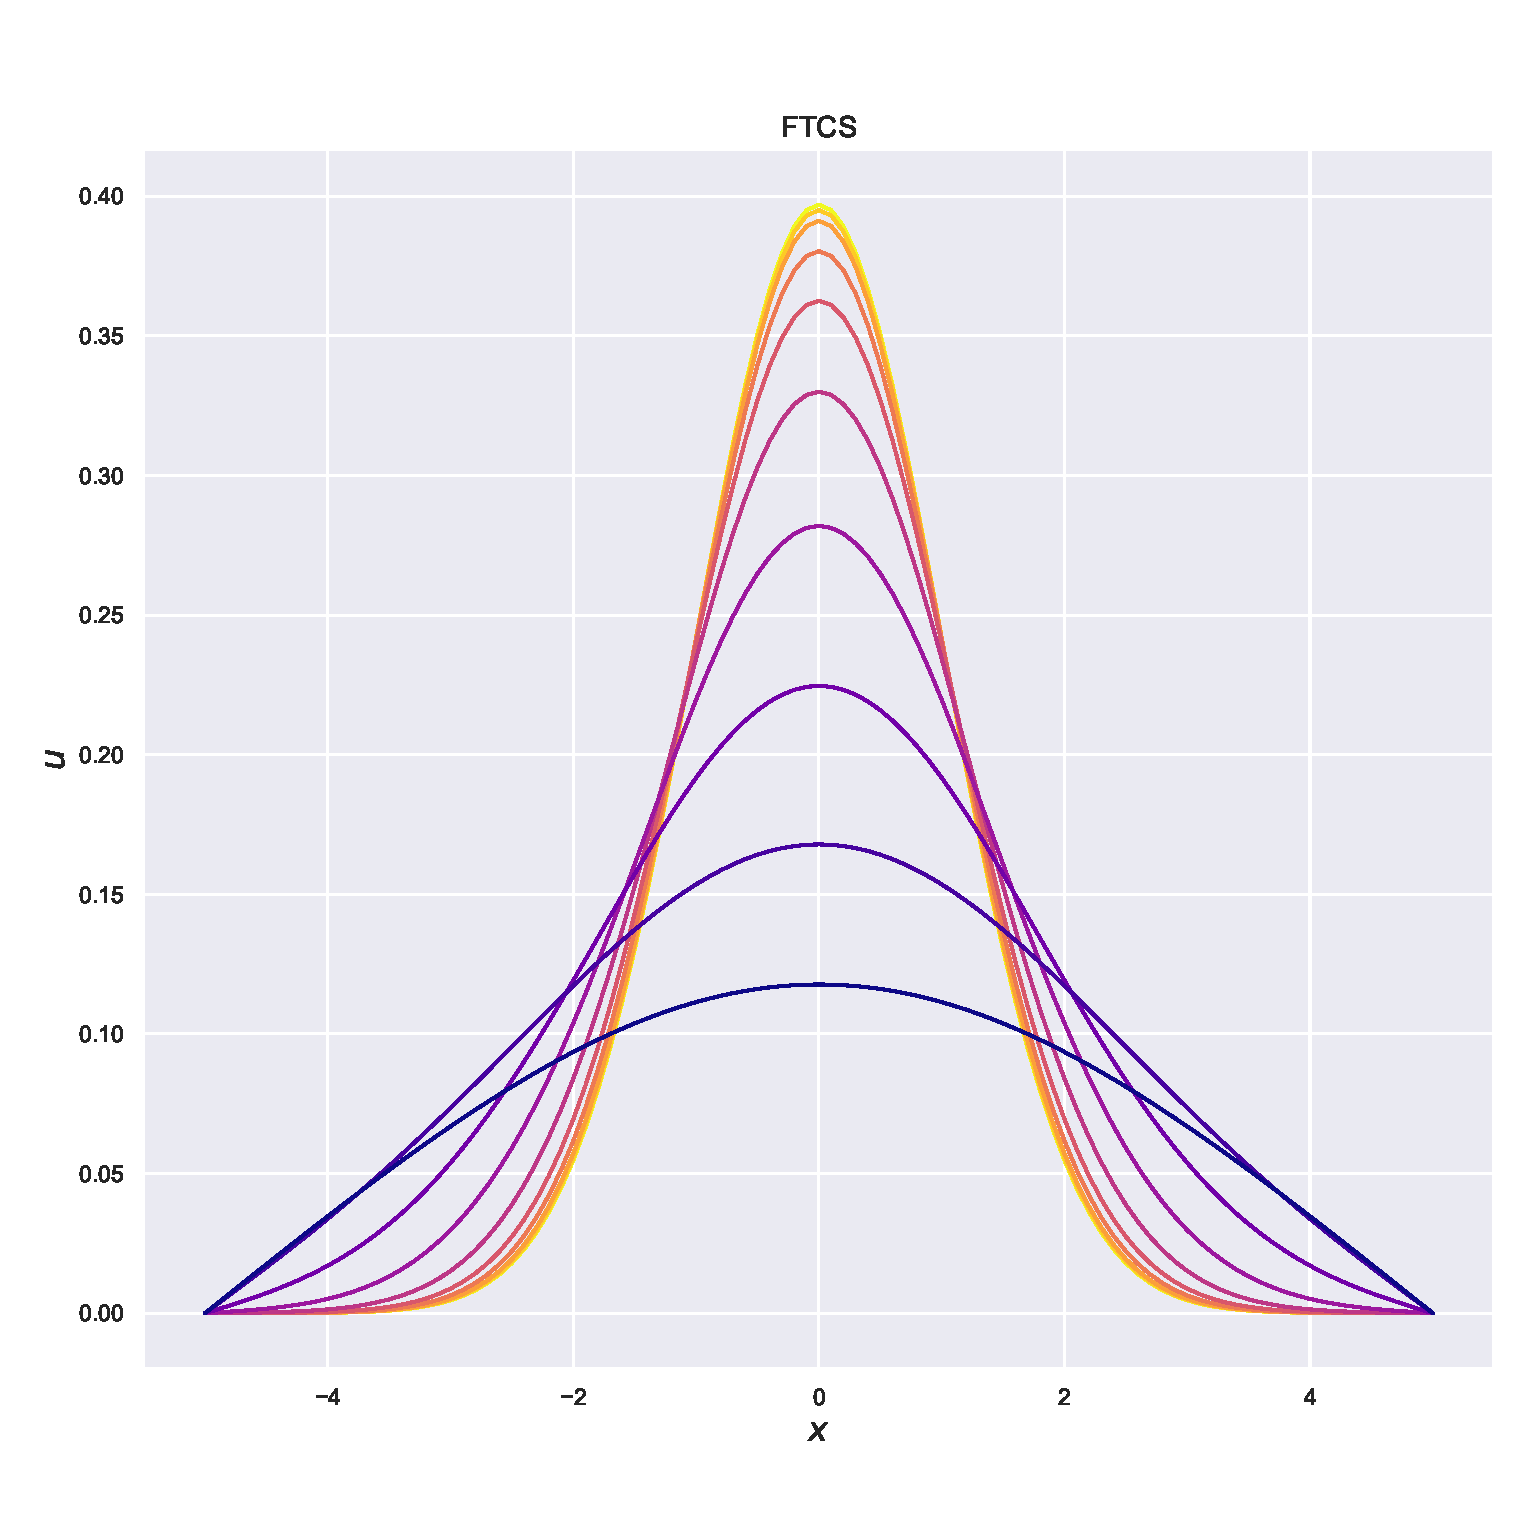
\includegraphics[width=\textwidth]{Figures/stableFTCSheat.eps}
                \subcaption{$\Delta t = 0.005$}
            \end{minipage} %
            \begin{minipage}[b]{0.49\textwidth}
                \centering
                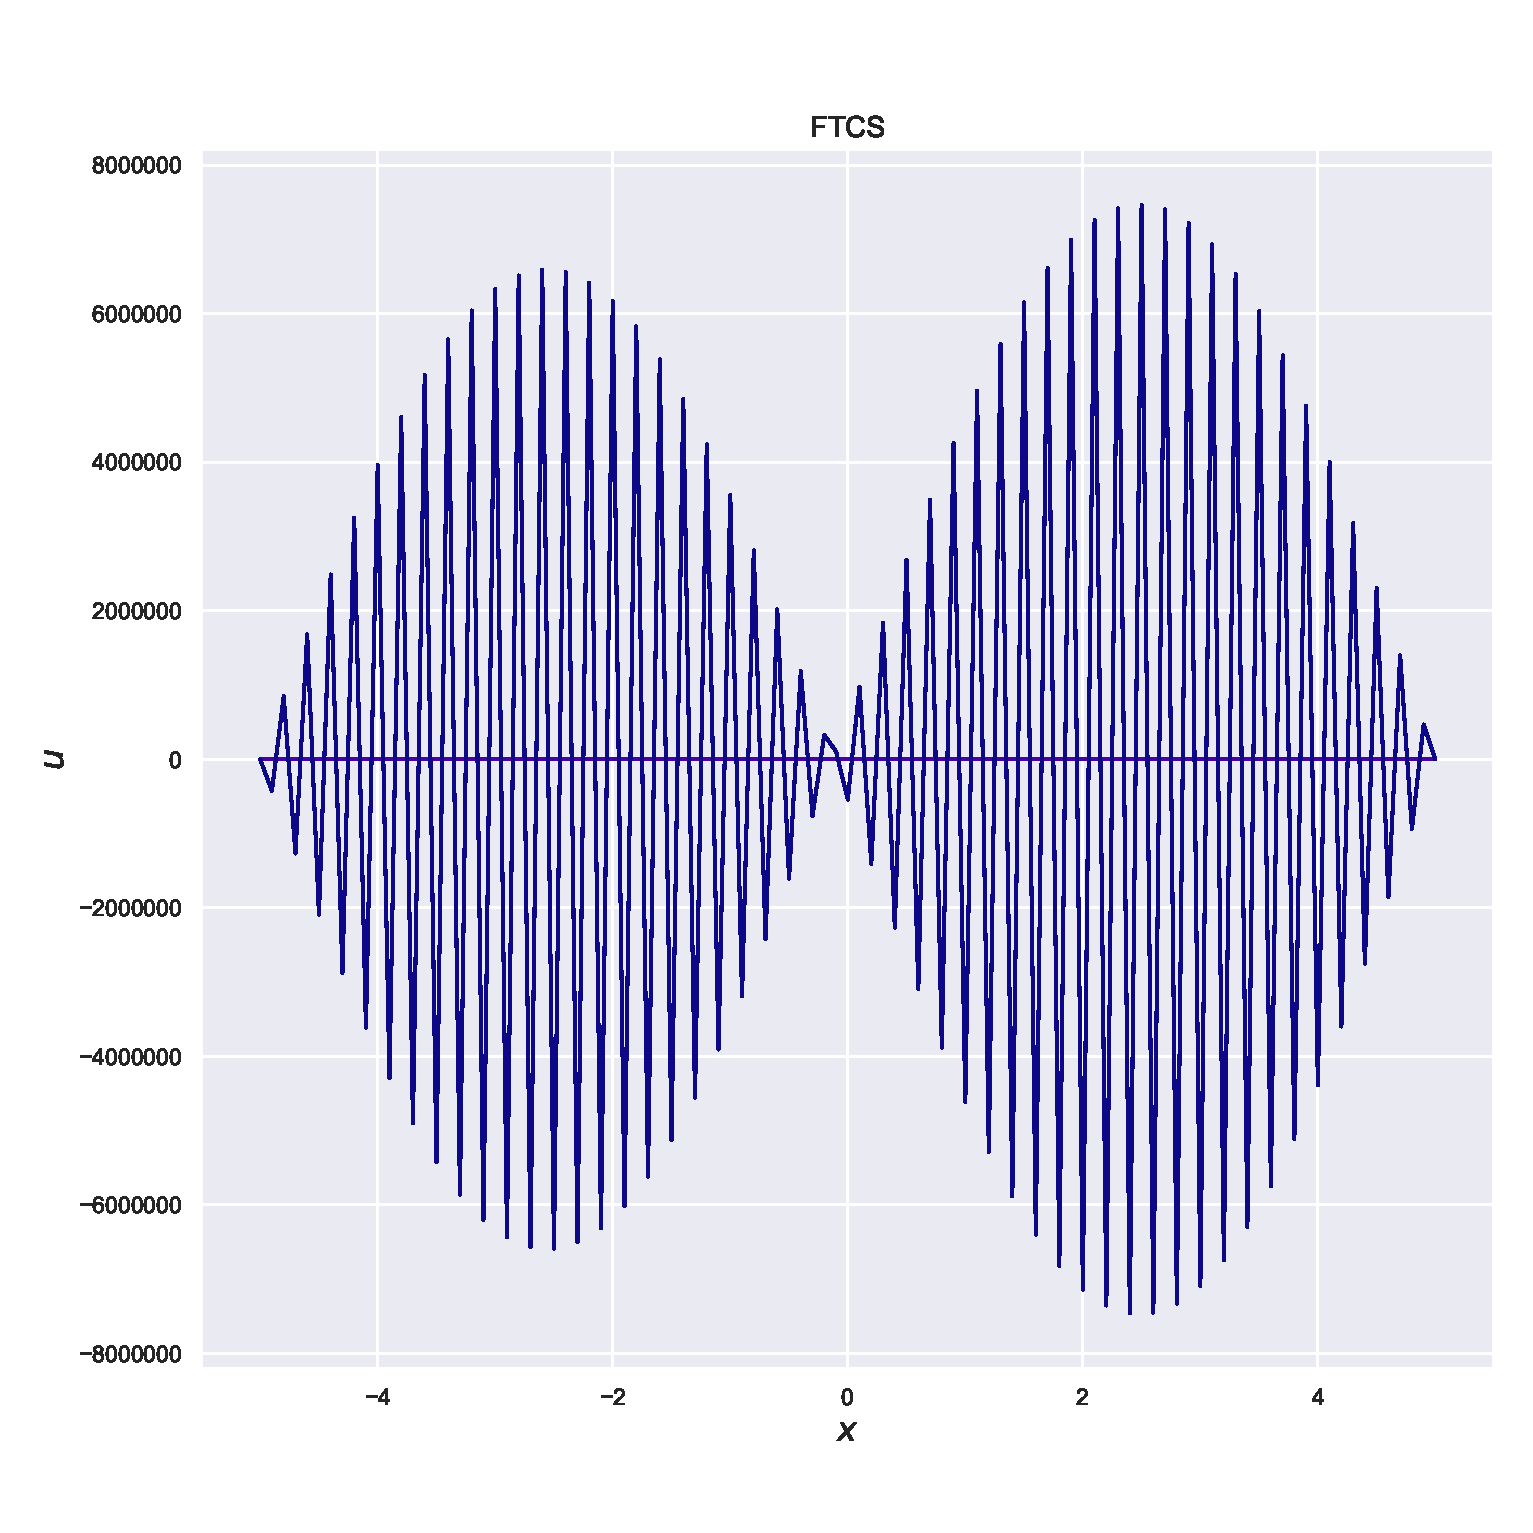
\includegraphics[width=\textwidth]{Figures/unstableFTCSheat.eps}
                \subcaption{$\Delta t = 0.0051$}
            \end{minipage} %
            \caption{Using the \texttt{FTCS} scheme to solve the heat equation \eqref{eq:heat} on $ \lbrack -5,5\rbrack \times\lbrack -1,1\rbrack$ with $\sigma =1, \Delta x = 0.1$ with a Gaussian initial profile.} 
            \label{fig:FTCSunstable}
        \end{figure}
        
        Of these two results, the stability condition is the greater concern. In the next section we look to new methods to remove any restrictions on the mesh spacing, whilst maintaining (or improving) the truncation error.
        
        \subsubsection*{Crank-Nicolson Method}
        To overcome the restriction in mesh spacing, one can use an implicit method, that is one where the solution depends on future time steps as well as the current. A method of this form is not as easy to solve, but as we will show here, has better accuracy and is unconditionally stable. The implicit Euler scheme appears the same as the explicit scheme above however here we calculate the spatial derivative at the future time step in place of the current one as follows:
        \[
          \frac{U^{n+1}_{j}  - U^{n}_{j}}{\Dt} = \sigma \frac{U^{n+1}_{j+1}-2U^{n+1}_{j}+U^{n+1}_{j-1}}{(\Dx)^2}
        \]
        The Crank-Nicolson scheme involves taking the average of the implicit and explicit schemes outlined so far:
        \[
             \frac{U^{n+1}_{j}-U^{n}_{j}}{\Dt} = \frac{\sigma}{2}\left(\frac{U^{n+1}_{j+1}-2U^{n+1}_{j}+U^{n+1}_{j-1}}{(\Dx)^2}+\frac{U^{n}_{j+1}-2U^{n}_{j}+U^{n}_{j-1}}{(\Dx)^2}\right)
        \]
        +++ picture of mesh+++
        Rearranging this equation so that all unknown quantities (future time steps) are on the left hand side gives,
            \[
                -\frac{\mu}{2} U^{n+1}_{j-1} + (1+\mu)U^{n+1}_{j} - \frac{\mu}{2} U^{n+1}_{j-1} = U^{n}_{j} + \frac{\mu}{2} \left( U^{n}_{j+1} - 2U^{n}_{j}+U^{n}_{j-1}\right),
            \]
        where $\mu = \frac{\sigma \Dt}{(\Dx)^2 }$. This is a tridiagonal system and can be reduced to an upper triangular matrix and solved using the Thomas algorithm\footnote{This is also known as the tridiagonal matrix algorithm}. Doing so removes the costly requirement of inverting a matrix.

        As for the stability of such a method, by applying the method seen for the fully-explicit scheme, one obtains 
        \[
            \lambda = \frac{1-2\mu\sin^2\left(\frac{k\Dx}{2}\right)}{1+2\mu\sin^2\left(\frac{k\Dx}{2}\right)}.
        \]
        Here $|\lambda| \not> 1$, so the method is unconditionally stable. We can also apply the same method as before to find the truncation error. Doing so gives that the Crank-Nicolson scheme is second-order in both time and space.
        \begin{figure}
            \centering
            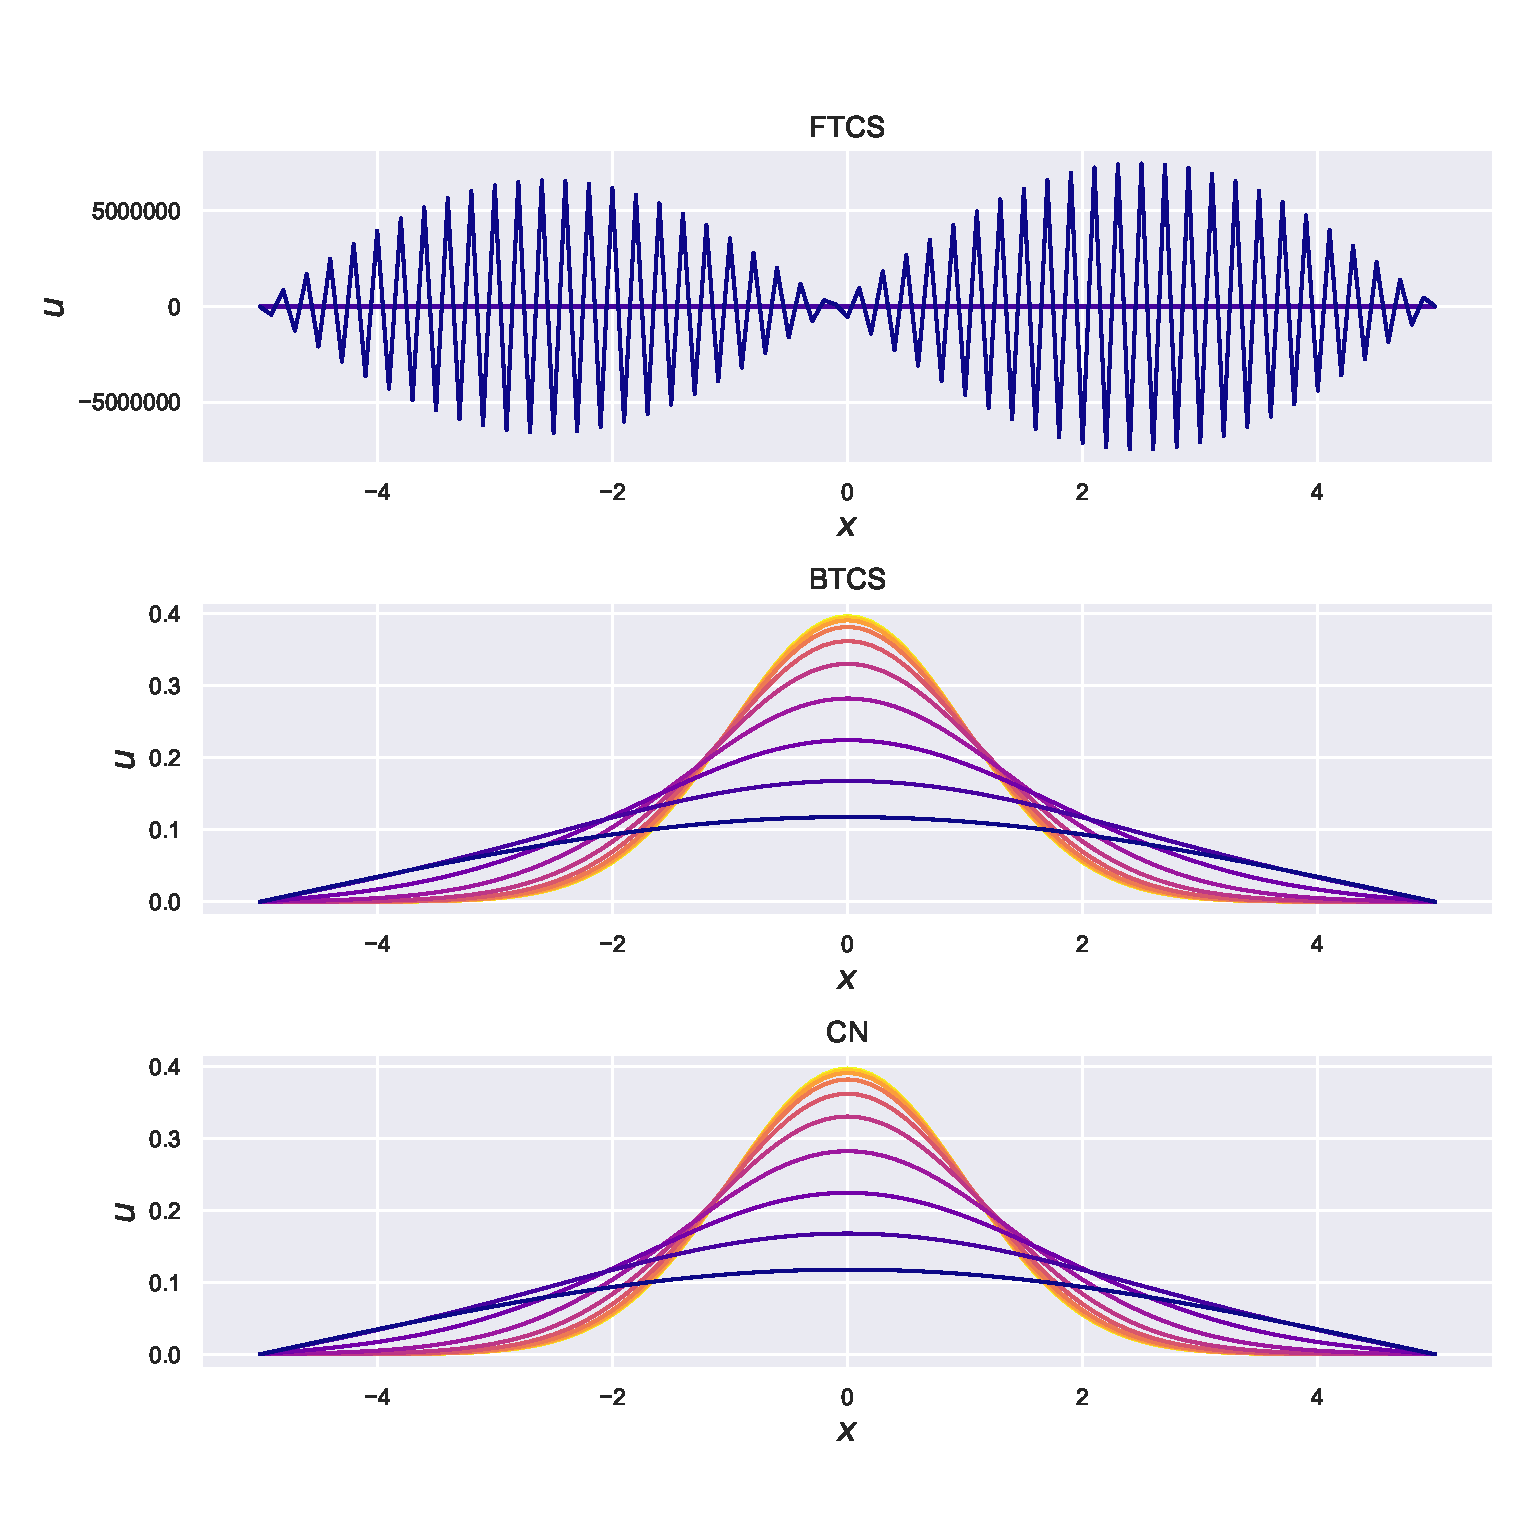
\includegraphics[width=0.7\linewidth]{Figures/FTCSandCN}
            \caption{Solving the heat equation as in Figure \ref{fig:FTCSunstable} using \texttt{FTCS, BTCS} and \texttt{CN} respectively. The implicit solvers remain stable regardless of step size.}
            \label{fig:ftcsandcn}
        \end{figure}
        
        \subsection{Advection Equations}
        Our prototypical example in this case will be the one-way wave equation,
        \begin{equation}\begin{cases}
            \partial_t u(t,x) + a\partial_x u(t,x)=0,\\
            u(0,x) = u_0(x),  &t\in\R^+, x\in\R.
        \end{cases}\label{eq:wave}\end{equation}
        Using the same discretisation as for the time derivative in the diffusion equation, yields the first order upwind scheme,
        \[
            \frac{U^{n+1}_{j}-U^{n}_{j}}{\Dt} = \begin{cases} a\frac{U^{n}_{j+1}-U^{n}_{j}}{\Dx} & \text{ if } a>0\\[0.5em]
                                                              a\frac{U^{n}_{j}-U^{n}_{j-1}}{\Dx} & \text{ if } a<0\\
                                                \end{cases}
        \]
        If the sign of \(a\) is not taken into account, the scheme is unstable. For further details see \cite{Hundsdorfer2007}.
        +++Error, modified equation showing dispersion +++
        
        \begin{figure}
            \centering
            \begin{minipage}[b]{0.49\textwidth}
                \centering
                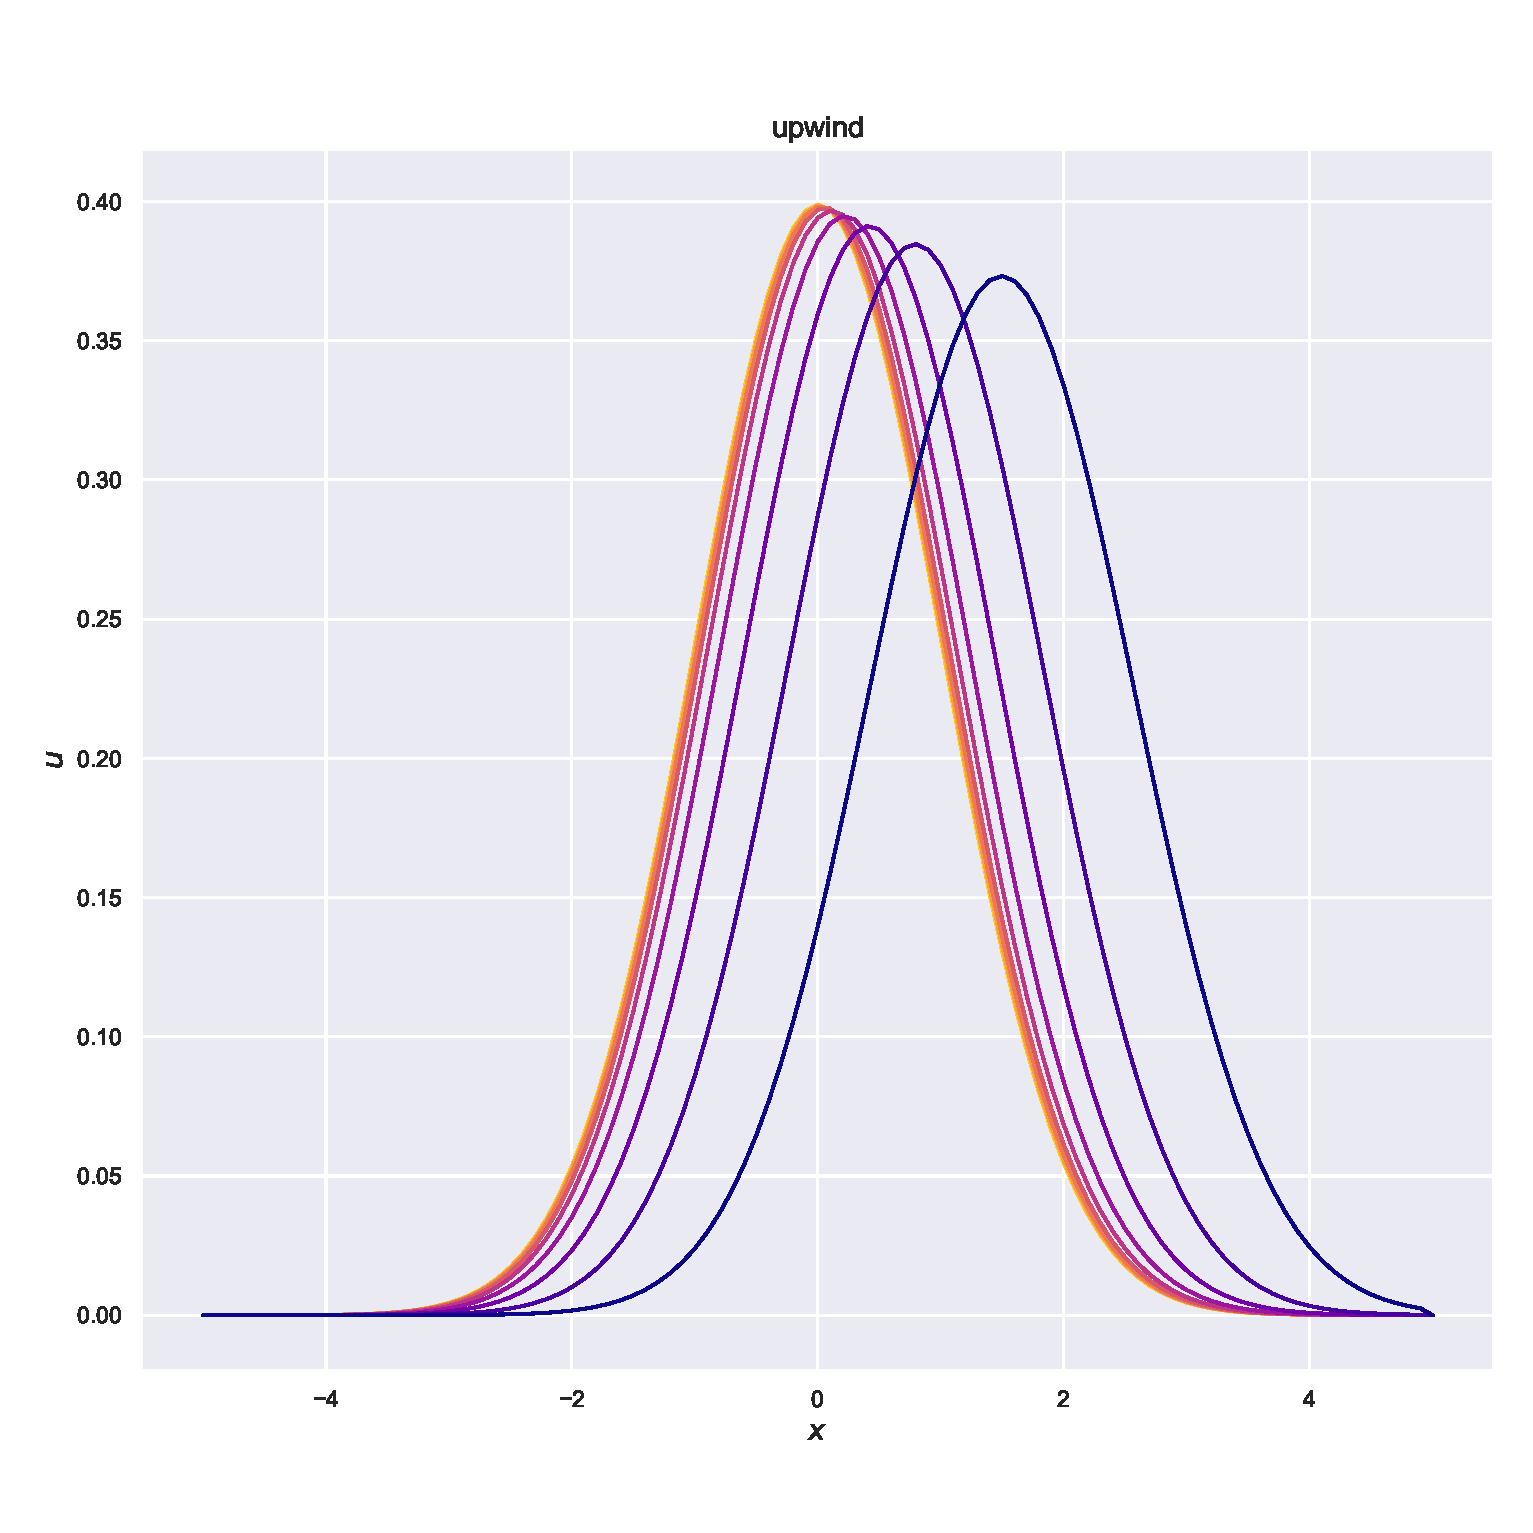
\includegraphics[width=\textwidth]{Figures/advgaussian.eps}
                \subcaption{$U_0 \sim \mathcal{N}(0,1)$}
            \end{minipage} %
            \begin{minipage}[b]{0.49\textwidth}
                \centering
                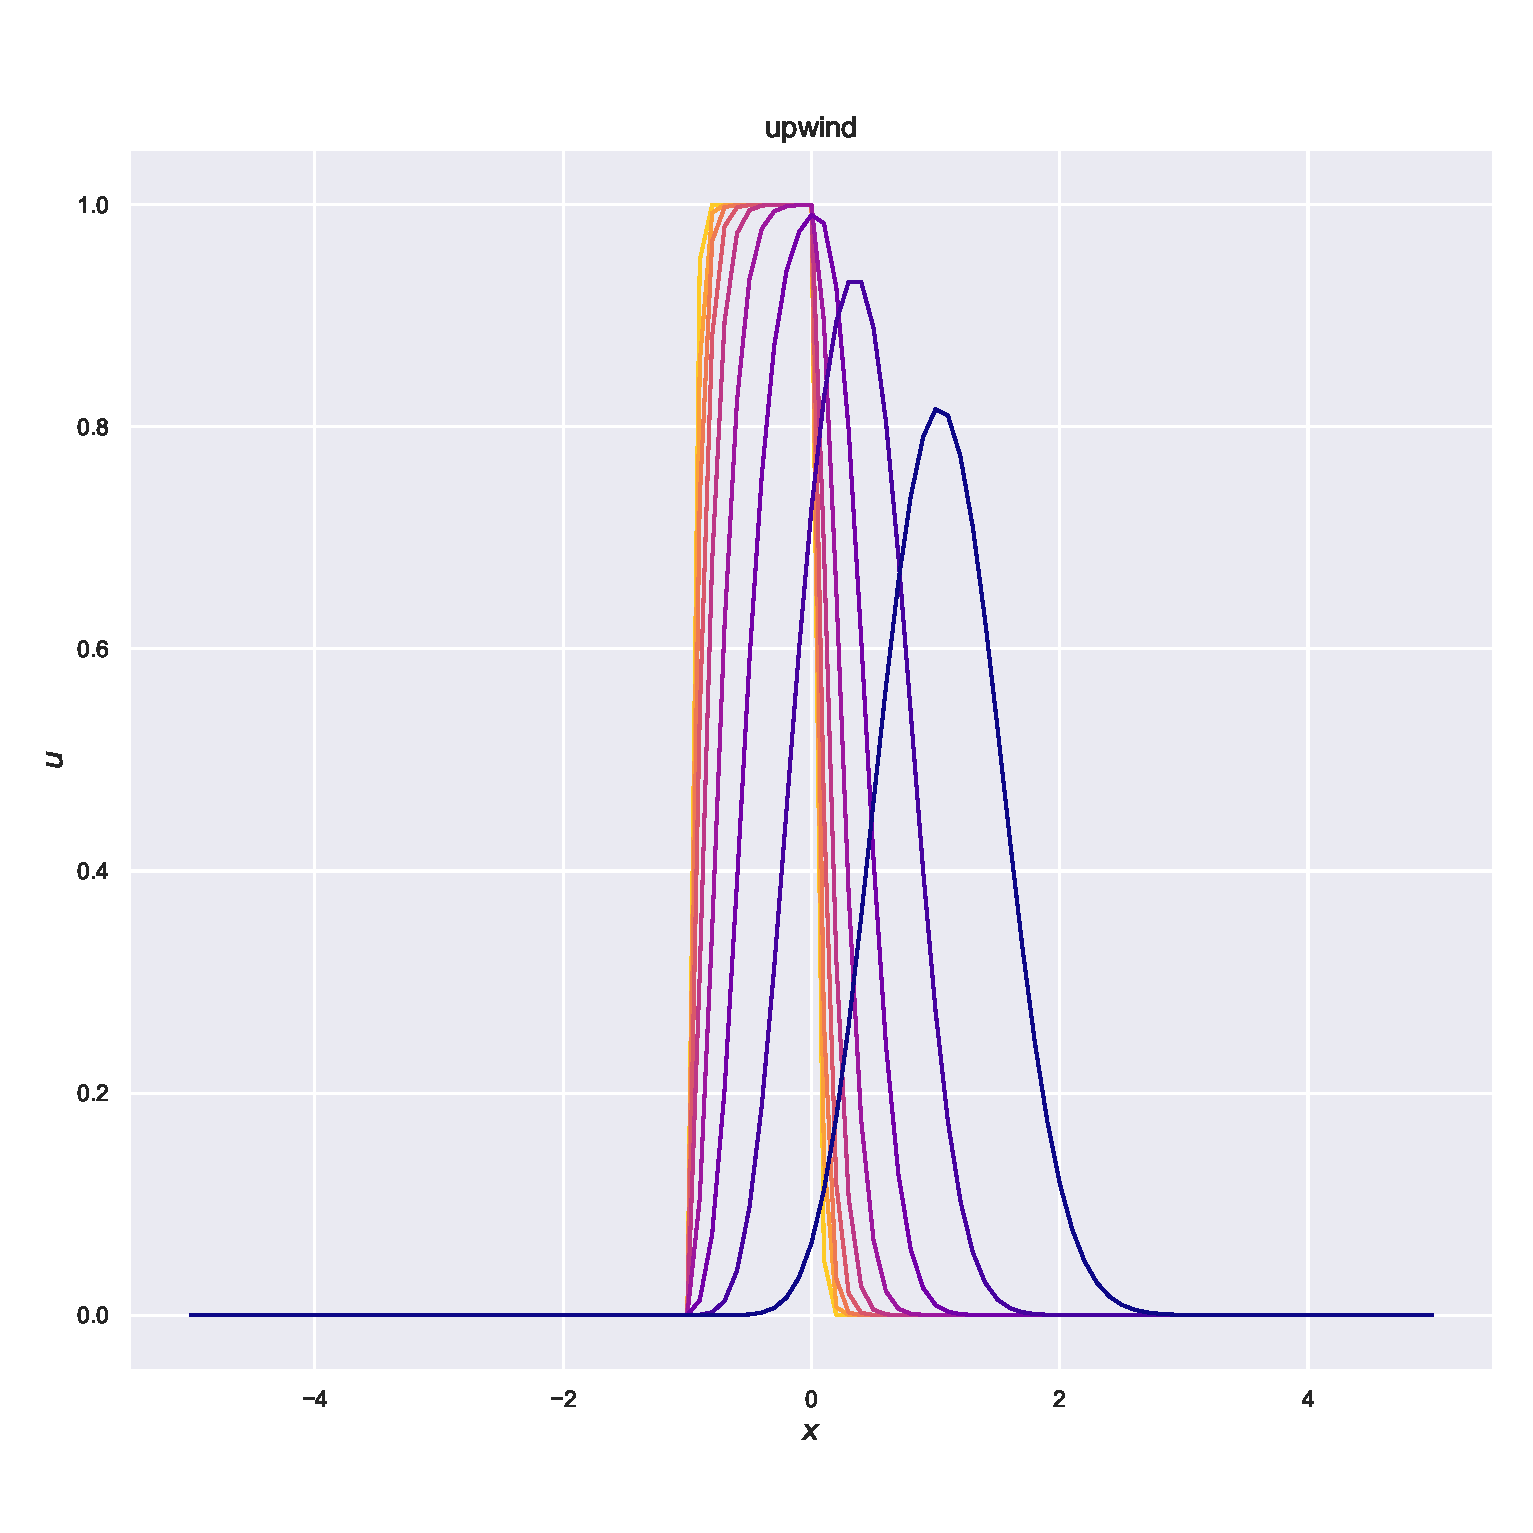
\includegraphics[width=\textwidth]{Figures/advindicator.eps}
                \subcaption{$U_0(x) = \mathbbm{1}_{\lbrack-1,0\rbrack}(x)$}
            \end{minipage} %
            \label{fig:advection}
            \caption{Solving equation \eqref{eq:wave} with the upwind scheme. Even with very smooth initial data, dispersive effects can be severe.} 
        \end{figure}
        \subsection{Particle Systems}
            Simulating particle systems requires the numerical solution of SDEs. The standard method for this is the Euler-Maruyama (EM) method, which can be seen as the stochastic analogue of Euler's method. Our motivating example here will be a system of particles moving according to an Ornstein-Uhlenbeck process\footnote{This is also the overdamped Langevin equation}. That is, a system of $N$ particles moving according to:
            \begin{equation}
                \dif x^{i,N}_t = - x^{i,N}_t \dif t + \sigma \dif W^i_t
            \end{equation}
            This is exactly the same as the space-homogeneous particle system \eqref{eq:hom_particle}, with no interaction between particles, and so provides the ideal starting point. Applying the EM method to the above equation gives:
            \[ x^{i,N}_{n+1} = x^{i,N}_n -  x^{i,N}_n\Dt + \sqrt{2\sigma\Dt}Z^i_n,  \]
		    where $Z_n$ is a standard normal random variable. This discretisation is very quick to compute, and has strong order $\frac{1}{2}$ \cite{Higham01}. As $N \to \infty$, the density of the particles will tend towards the solution to the evolution given by \eqref{eq:hom_particle}, as we will see in Section +++REF+++. This gives us a method of finding the stationary distribution: simulate many particles for a long time. Eventually, the density of the particles will be approximately the stationary distribution of the system\footnote{It is in fact not even necessary to simulate many particles -- if the system is allowed to evolve for long enough, one particle will suffice.}. The particle system will be an excellent metric by which to test the schemes developed for the continuum models.
            \begin{figure}
                \centering
                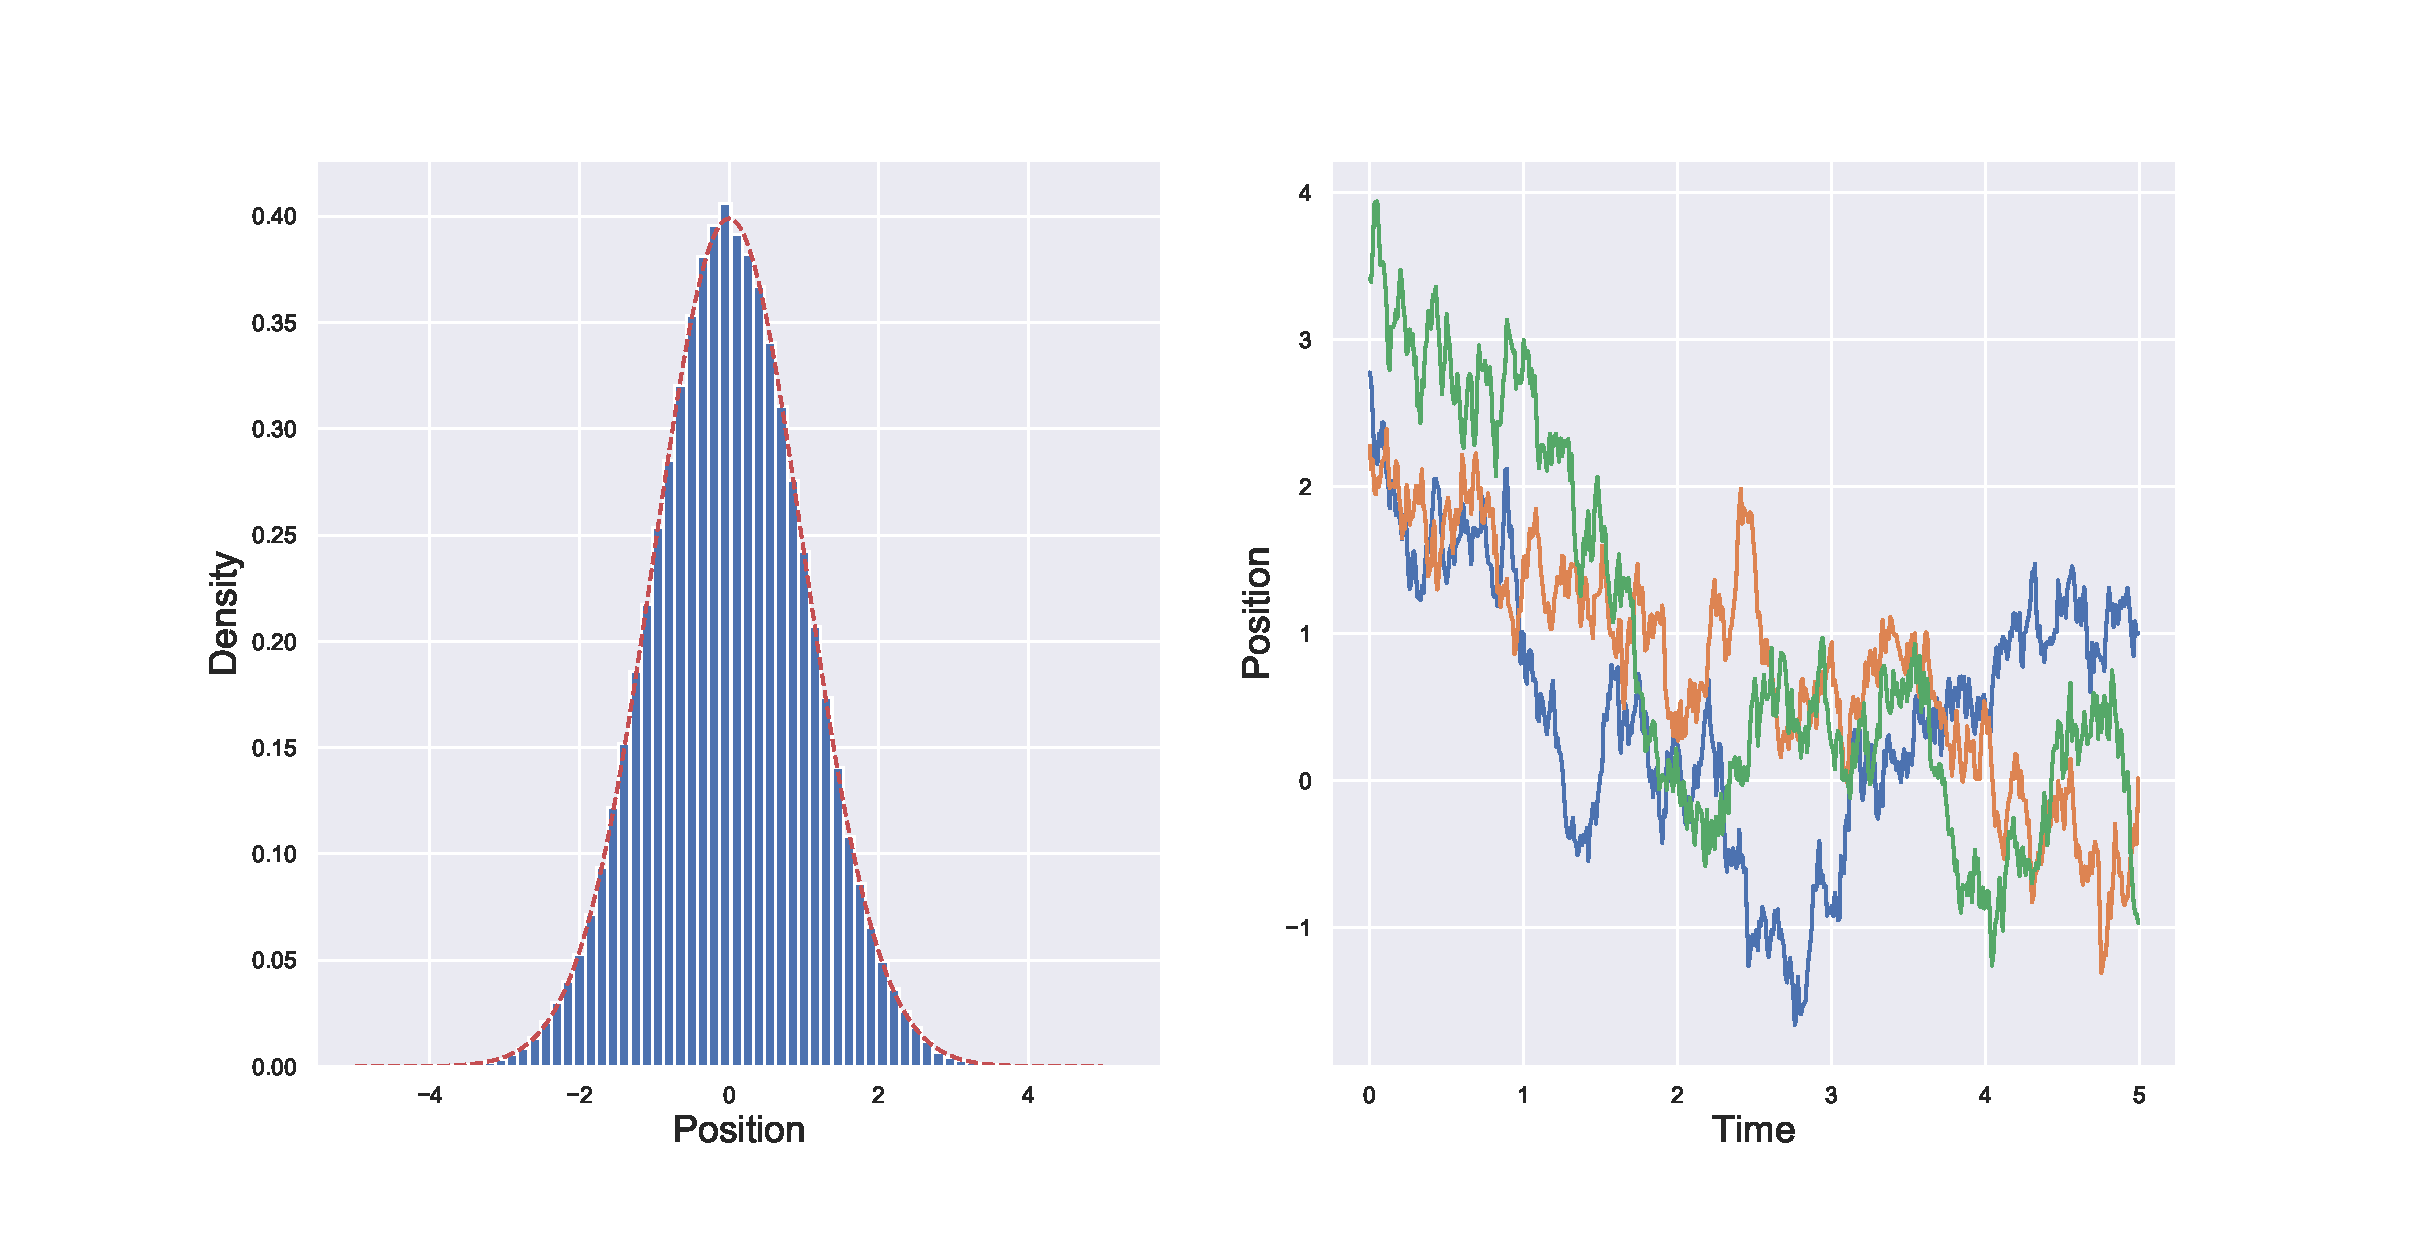
\includegraphics[width=0.7\linewidth]{Figures/OUparticletraj}
                \caption{Histogram of positions of 1000 particles after 100s with $\sigma = 1$, and positions of 5 particles over time.}
                \label{fig:ouparticletraj}
            \end{figure}
            
		\section{Applying the Numerical Scheme}
			We now have enough techniques to begin solving the kinetic model. Consider the space-homogeneous evolution given by \eqref{eq:space_hom_PDE}, that is
			\begin{equation}
				\partial_t f_t(v) = \partial_v vf_t(v) - \partial_v G(\langle w \rangle_{f_t})f_t(v) + \sigma \partial_{vv} f_t(v).
			\end{equation}
            Using the methods developed in the previous section, we are now able to solve this system numerically. As when solving the heat equation, a zero boundary condition shall be enforced. This is valid as we know that the stationary distributions are Gaussian and centred at $-1,0,+1$. The boundary $L$ can then be chosen depending on the the diffusion so that almost no mass is contained beyond the boundary. For example if $\sigma = 1$, the mass contained beyond $L=5$ is of the order $10^{-5}$. 
            
			Simpson's rule will be used as a quick way to approximate the integral within the herding coefficient. To differentiate between the integral and its approximation, we write \(\langle w\rangle_{F^n}\). Below is the scheme when both the herding coefficient and the velocity are positive, using a finite difference scheme with a CN discretisation for the diffusive term and an upwind method for the damping and herding terms.
			\begin{equation*}
			\begin{split}
				\frac{F_j^{n+1} - F_j^n}{\Delta t} = 	-G(\langle w\rangle_{F^n})\left[ \frac{F^n_{j+1} - F^n_{j}}{\Delta v}\right] &+\left[ \frac{v_{j}F^n_{j} - v_{j-1}F^n_{j-1}}{\Delta v}\right]\\ &+ \frac{\sigma}{2}\left[ \frac{F^{n+1}_{j+1} - 2F^{n+1}_j + F^{n+1}_{j-1}}{(\Delta v)^2} + \frac{F^{n}_{j+1} - 2F^{n}_j + F^{n}_{j-1}}{(\Delta v)^2}\right] 	 
			\end{split}
			\end{equation*}

			+++Pictures, moments converging, error (in moments too?) in particular, mass loss? -> compare conservative methods i.e. fin vol +++
        \subsection{Finite Volume Schemes}
            In Section \ref{sec:dynamics}, equations were closed on the moments of the distribution. From this, we know that \(\dot{M}_0 = 0\), that is mass is conserved. This suggests that numerical schemes designed to conserve mass would be ideal for solving this system. One such method is a finite volume scheme, a generalisation of finite difference methods. First, we write the system in conservative form. This is an equation of the form $\partial_ u = \partial_x(a(x)u)$. For the space homogenous model \eqref{eq:space_hom_PDE}, this corresponds to
            \begin{equation}\label{eq:flux_space_hom}
                \partial_t f_t = \partial_v \left[\left(v-G(\langle w \rangle_{f_t})\right)f_t + \sigma \partial_v f_t \right].
            \end{equation}
            Using the same discretisation as in Section \ref{sec:numericalmethods}, we further introduce auxiliary points $v_{j\pm\frac{1}{2}} = \frac{1}{2}(v_{j\pm1} + v_j) $. Then within any cell (or volume), $\Omega_j = [v_{j-\frac{1}{2}}, v_{j+\frac{1}{2}}]$, we can calculate the average.
            \[
                 \bar{f}_t(v_j) = \frac{1}{\Dv}\int_{\Omega_j} f_t(v) \dif v = f_t(v_j)+\frac{1}{24(\Dv)^2} \partial_{vv} f_t(v_j)
             \]
            Furthermore, the change in the average density within the cell is equal to difference of the mass lost through either side of the volume, that is,
            \[
                \Dv\od{\bar{f}_t(v_j)}{t} = a(v_{j-\frac{1}{2}})f_t(v_{j-\frac{1}{2}}) - a(v_{j-\frac{1}{2}})f_t(v_{j-\frac{1}{2}}), 
            \]
            where $a(v) = \left[\left(v-G(\langle w \rangle_{f_t(v)})\right)f_t + \sigma \partial_v f_t(v) \right]$. This can then be approximated using a finite volume scheme:
            \[
                \frac{F^{n+1}_j - F^n_j}{\Dt} = \frac{1}{\Dv}\left[ a(v_{j-\frac{1}{2}})F^n_{j-\frac{1}{2}} - a(v_{j-\frac{1}{2}})F^n_{j-\frac{1}{2}}\right]
            \]
            This is the first-order upwind scheme in conservative (flux) form. As in the previous upwind scheme, the choice of spatial points at which to evaluate depends on the sign of the advection term. That is,
            \[
                a(v_{j+\frac{1}{2}})F^n_{j+\frac{1}{2}} = a^+(v_{j+\frac{1}{2}})F^n_{j} + a^-(v_{j+\frac{1}{2}})F^n_{j+1},
            \]
            where $a^+ = \max(a,0), a^- = \min(a,0)$.  This scheme is still order 1, however it provides the ideal setting for developing higher order schemes.
            +++show agreement with FD, particle,  show symmetry in error+++
        \subsection{Space Heterogeneous}
        +++ phi = 1 still, moving in space. Animations/diagrams showing Leb in space. +++
        
        \section{Discussion + Conclusion}
        +++ future add other phi, recalc M +++
	\bibliographystyle{abbrv}
	\bibliography{whales.bib}
	\appendix

\end{document}